\section{Einleitung}

\begin{frame}
  \centering{\textbf{Problemdemonstration}}
\end{frame}

\begin{frame}[fragile]
  \frametitle{OpenAPI}
  \begin{itemize}
    \item Spezifikationsstandard für HTTP Schnittstellen
  \end{itemize}
  \lstset{language=none}
  \begin{lstlisting}[
    gobble=0,
    frame=none,
    captionpos=b,
    basicstyle=\footnotesize\ttfamily,,
    caption={Auszug aus dem Datensatz der Linterergebnisse},
    label={lst:rawdataexample},
  ]
  paths:
  /pet:
    put:
      requestBody:
        content:
          application/json:
            schema:
              $ref: '#/components/schemas/Pet'
        required: true
      responses:
        '200':
          description: Successful operation
  \end{lstlisting}
\end{frame}

\begin{frame}
  \frametitle{Linting OpenAPI}
  \begin{itemize}
    \item Erkennen möglicher Fehler mit statischer Code Analyse
    \item Spectral ist beliebter Linter für OpenAPI
    \item Standard Spectral Regelwerk für OpenAPI
  \end{itemize}
  Noch etwas mehr über Spectral Regeln oder Ruleset?
\end{frame}

\begin{frame}
  \frametitle{APIs.guru}
  \begin{itemize}
    \item Online Repository für OpenAPI Spezifikationen
    \item Qualitative, praxisnahe und kuratierte Spezifikationen
  \end{itemize}
  \hspace{1cm}
  \begin{columns}
    \begin{column}{0.5 \textwidth}
      \begin{figure}[htbp]
        \centering
        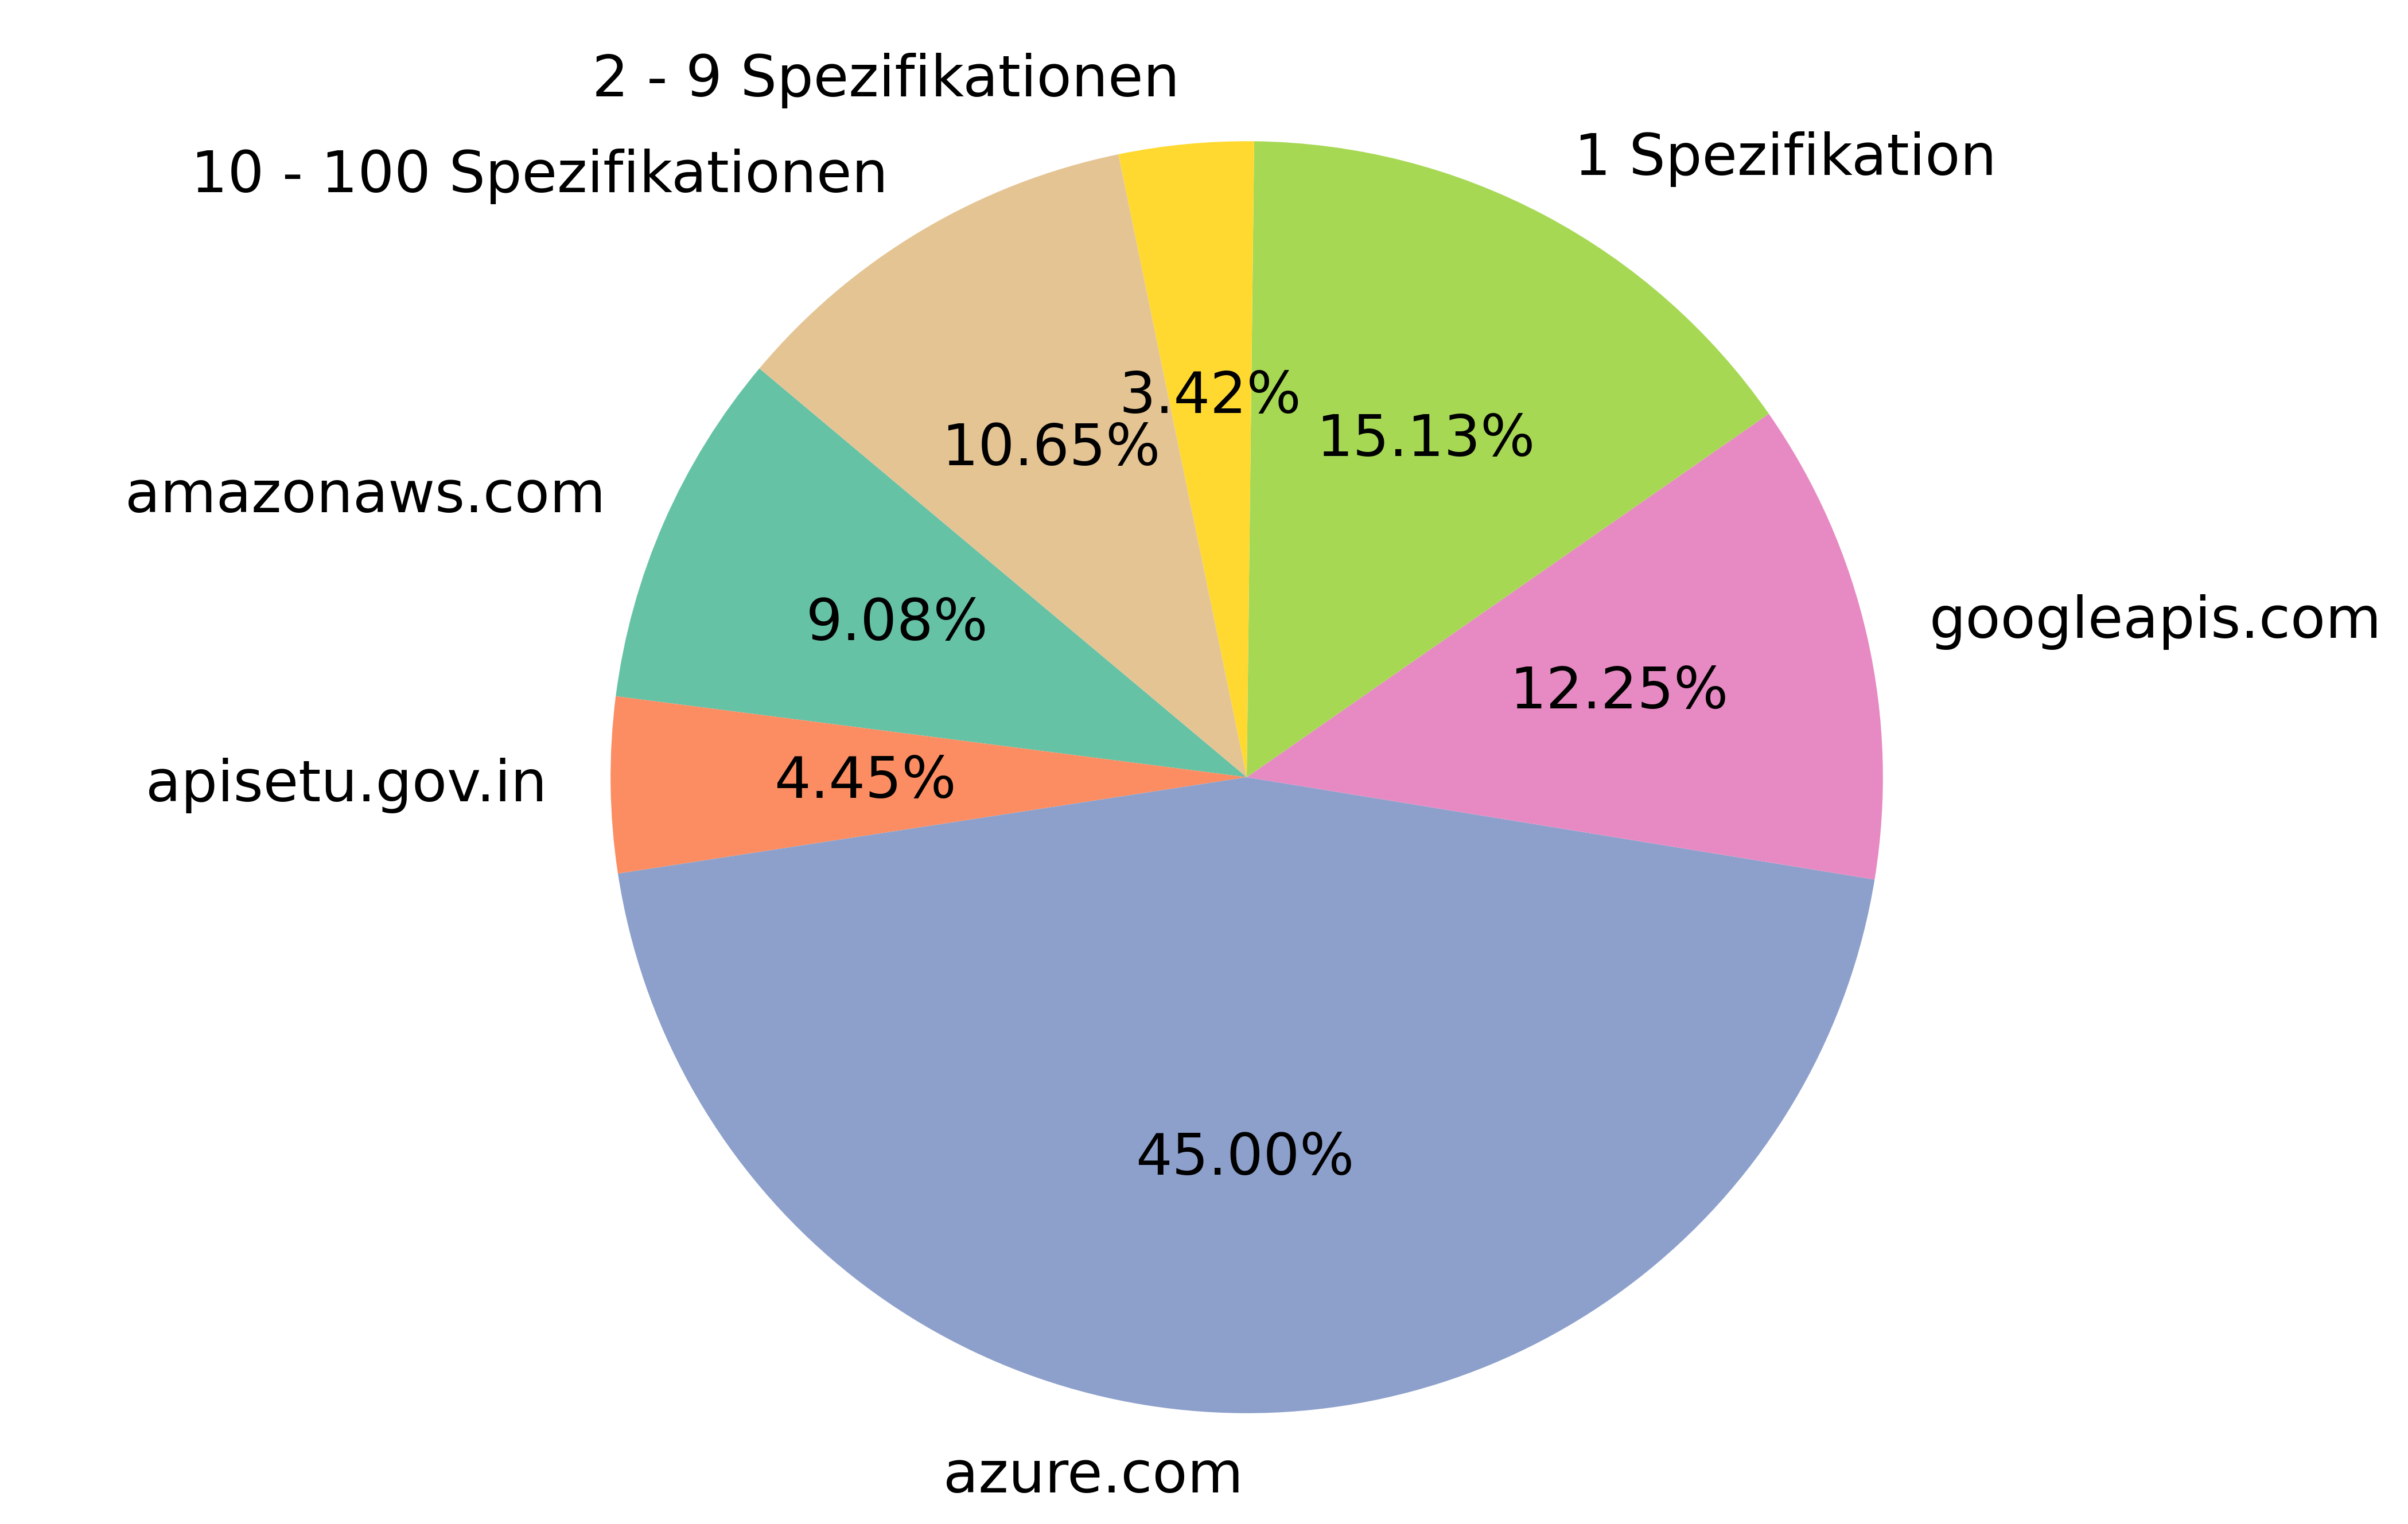
\includegraphics[width=1\textwidth]{images/specificationsperdomainpie.png}
        \caption{Anzahl der Spezifikationen pro Anbieter}
        \label{fig:Specifications}
      \end{figure}    
    \end{column}
    \begin{column}{0.5 \textwidth}
      \begin{figure}[htbp]
        \centering
        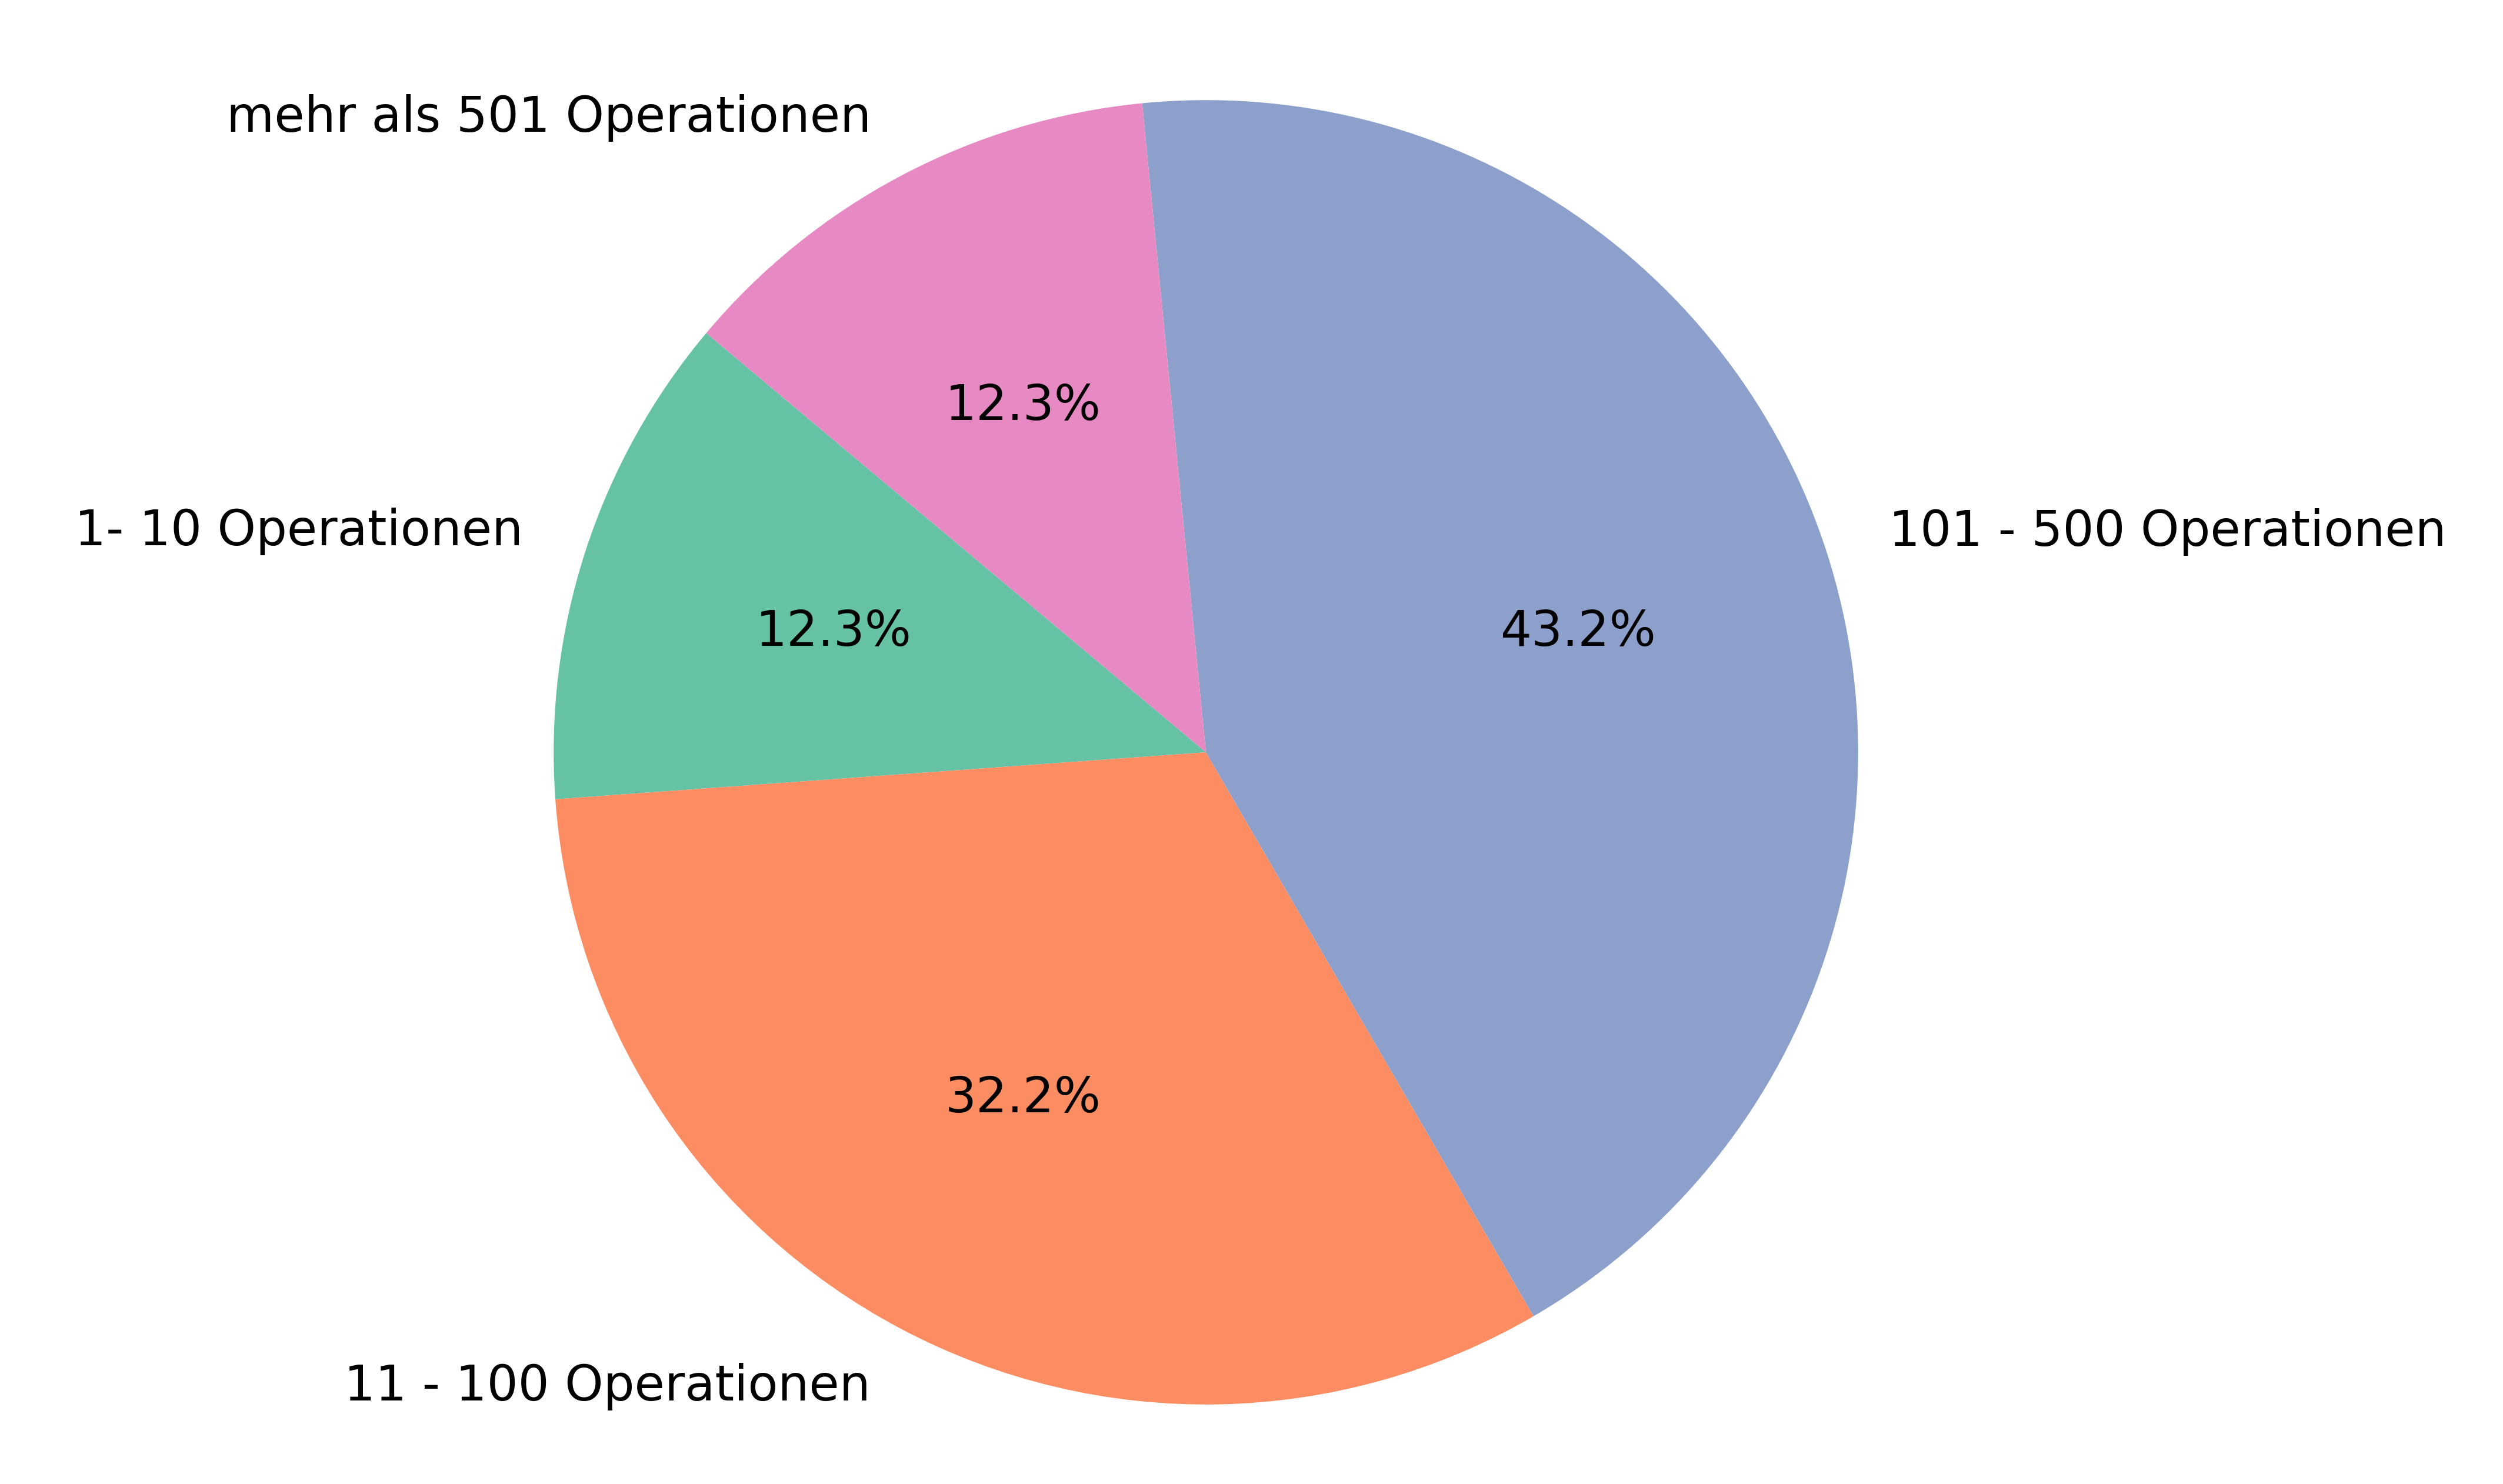
\includegraphics[width=1\textwidth]{images/operationsperspecificationpie.png}
        \caption{Anzahl der API Operationen pro Spezifikation}
        \label{fig:Operations}
      \end{figure}    
    \end{column}
  \end{columns}
\end{frame}


\section{Methodik}

\begin{frame}
  \frametitle{Linting}
  \vspace{-0.5cm}
  \begin{figure}[htbp]
    \centering
    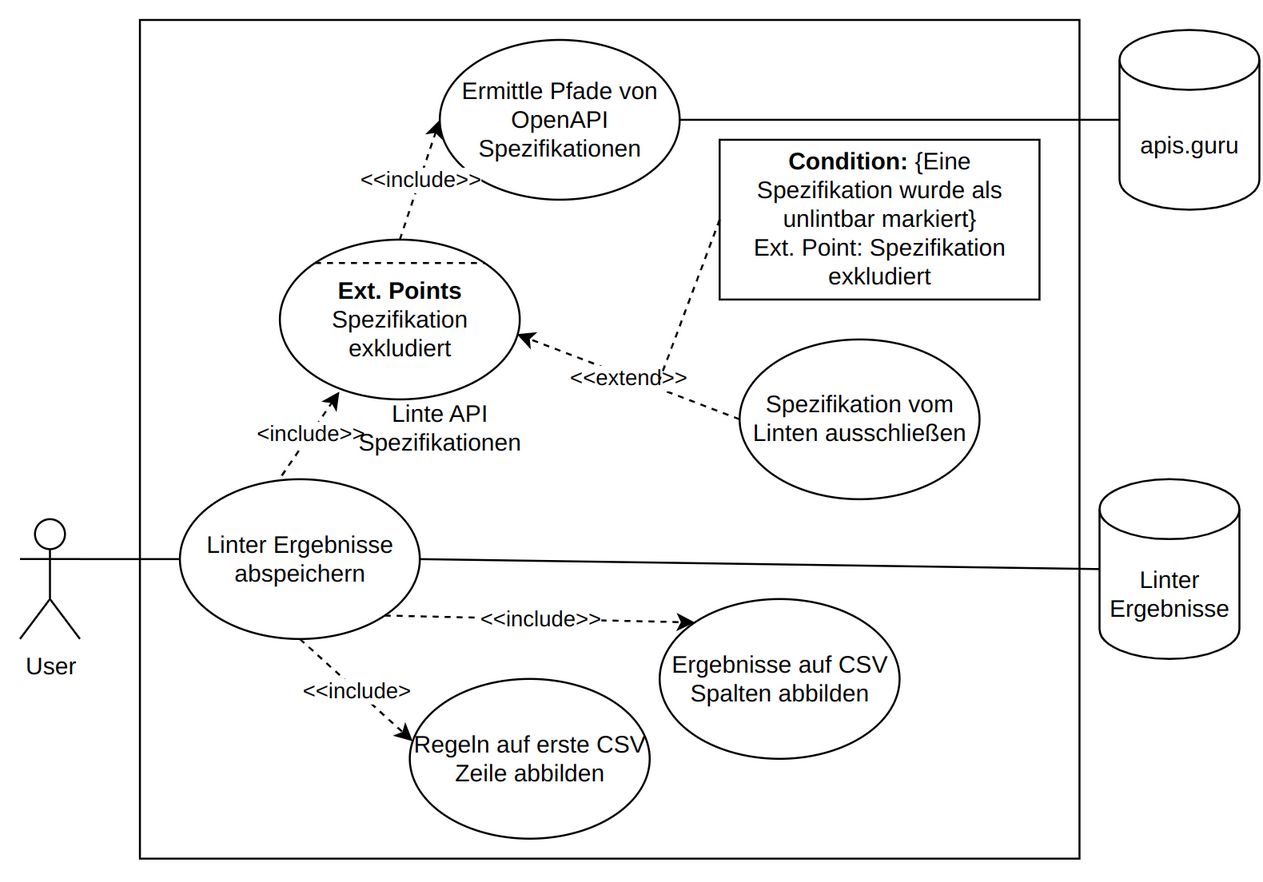
\includegraphics[width=0.9\linewidth]{images/linting.png}
    \caption{\textbf{UC-1} Linting}
    \label{fig:linting}
  \end{figure}
\end{frame}

\begin{frame}
  \frametitle{Invertierung}
  \vspace{-0.5cm}
  \begin{figure}[htbp]
    \centering
    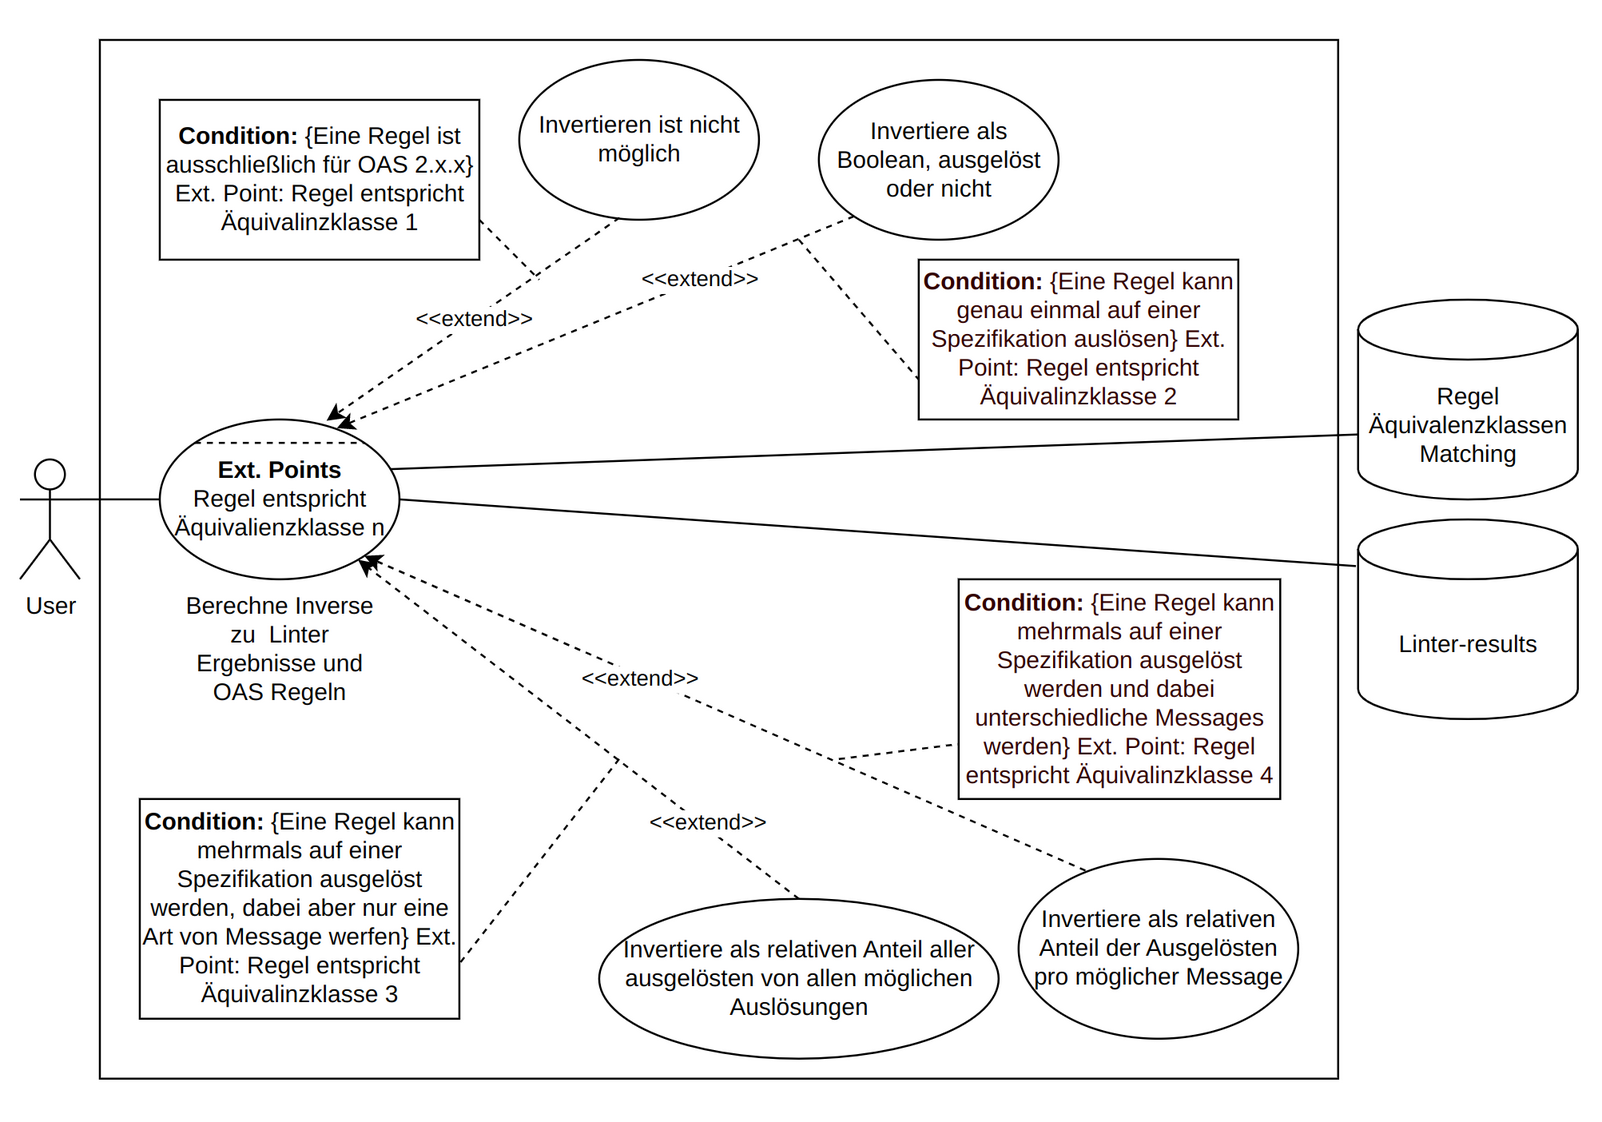
\includegraphics[width=0.9\linewidth]{images/invert.png}
    \caption{\textbf{UC-2} Invertierung}
    \label{fig:invert}
  \end{figure}
\end{frame}

\begin{frame}
  \frametitle{Softwarearchitektur}
  \vspace{-0.5cm}
  \begin{figure}[htbp]
    \centering
    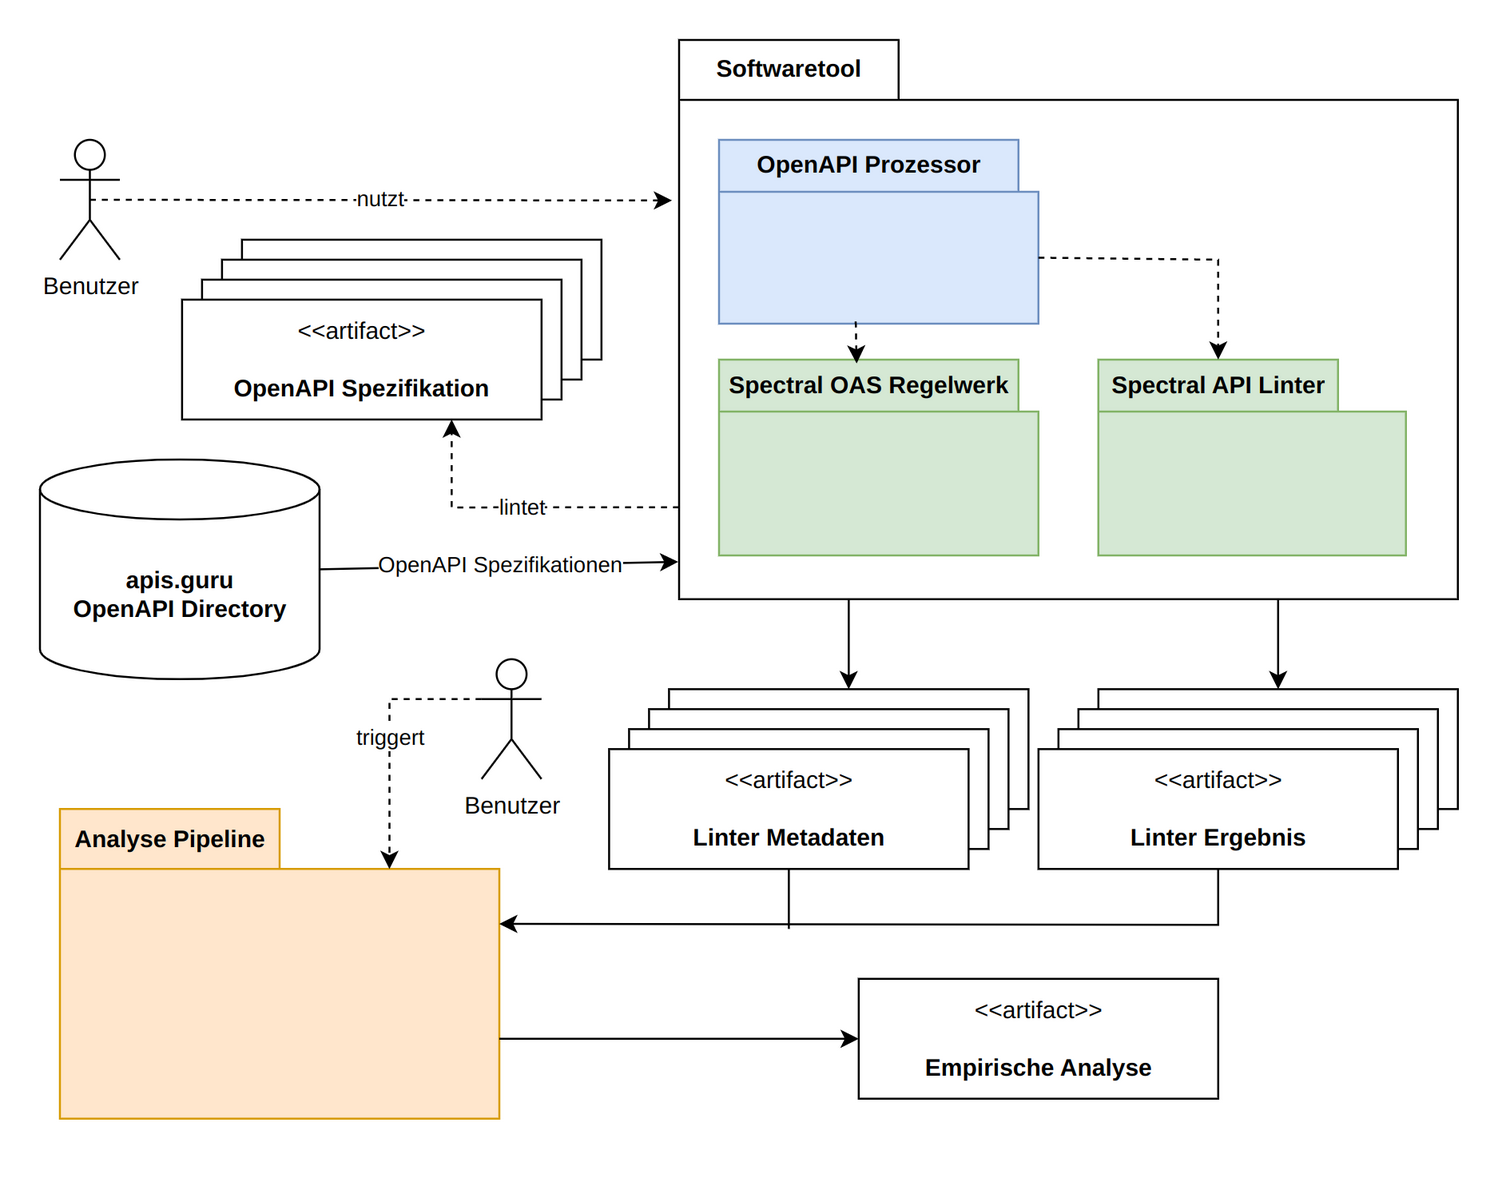
\includegraphics[width=0.8\linewidth]{images/contextview.png}
    \caption{Kontextsicht des Systems}
    \label{fig:Kontextsicht}
  \end{figure}
\end{frame}

\begin{frame}
  \frametitle{Priorisierung}
    \begin{greyblock}{Relevanz Frequenz}
      \scriptsize{
        \[
          \text{Relevanz}_\text{Frequenz}(r) = 
          \begin{cases}
          1&\text{, wenn } 0 = \sum_{i=1}^{n}vorkommen(r, i) \\
          \frac{1}{\sum_{i=1}^{n}vorkommen(r, i)}&\text{, sonst}.
          \end{cases}
        \]
        \[
          vorkommen(r, s) = 
          \begin{cases} 
          1&\text{, wenn die Spezifikation } s \text{ die Regel } r \text{ ausgelöst hat}, \\
          0&\text{, sonst}.
          \end{cases}
        \]
      }
    \end{greyblock}
    \begin{greyblock}{Relevanz Diversität}
      \scriptsize{
        \[
          \text{Relevanz}_\text{Diversität}(r) = (\frac{1}{n} \sum_{i=1}^{n} 1- Jaccard(r, r_i))
        \]
        \[
          Jaccard(A,B)=\frac{\vert A \cap B \vert}{\vert A \vert + \vert B \vert - \vert A \cap B \vert}
        \]
      }      
    \end{greyblock}
\end{frame}


\section{Analyse}

\begin{frame}
  \frametitle{Ergebnisse}
  \vspace{-0.4cm}
  \begin{itemize}
    \item 929.699 Linterfehler
    \item 7.778.972 mögliche Stellen für Linterfehler
  \end{itemize}
  \begin{figure}[htbp]
    \centering
    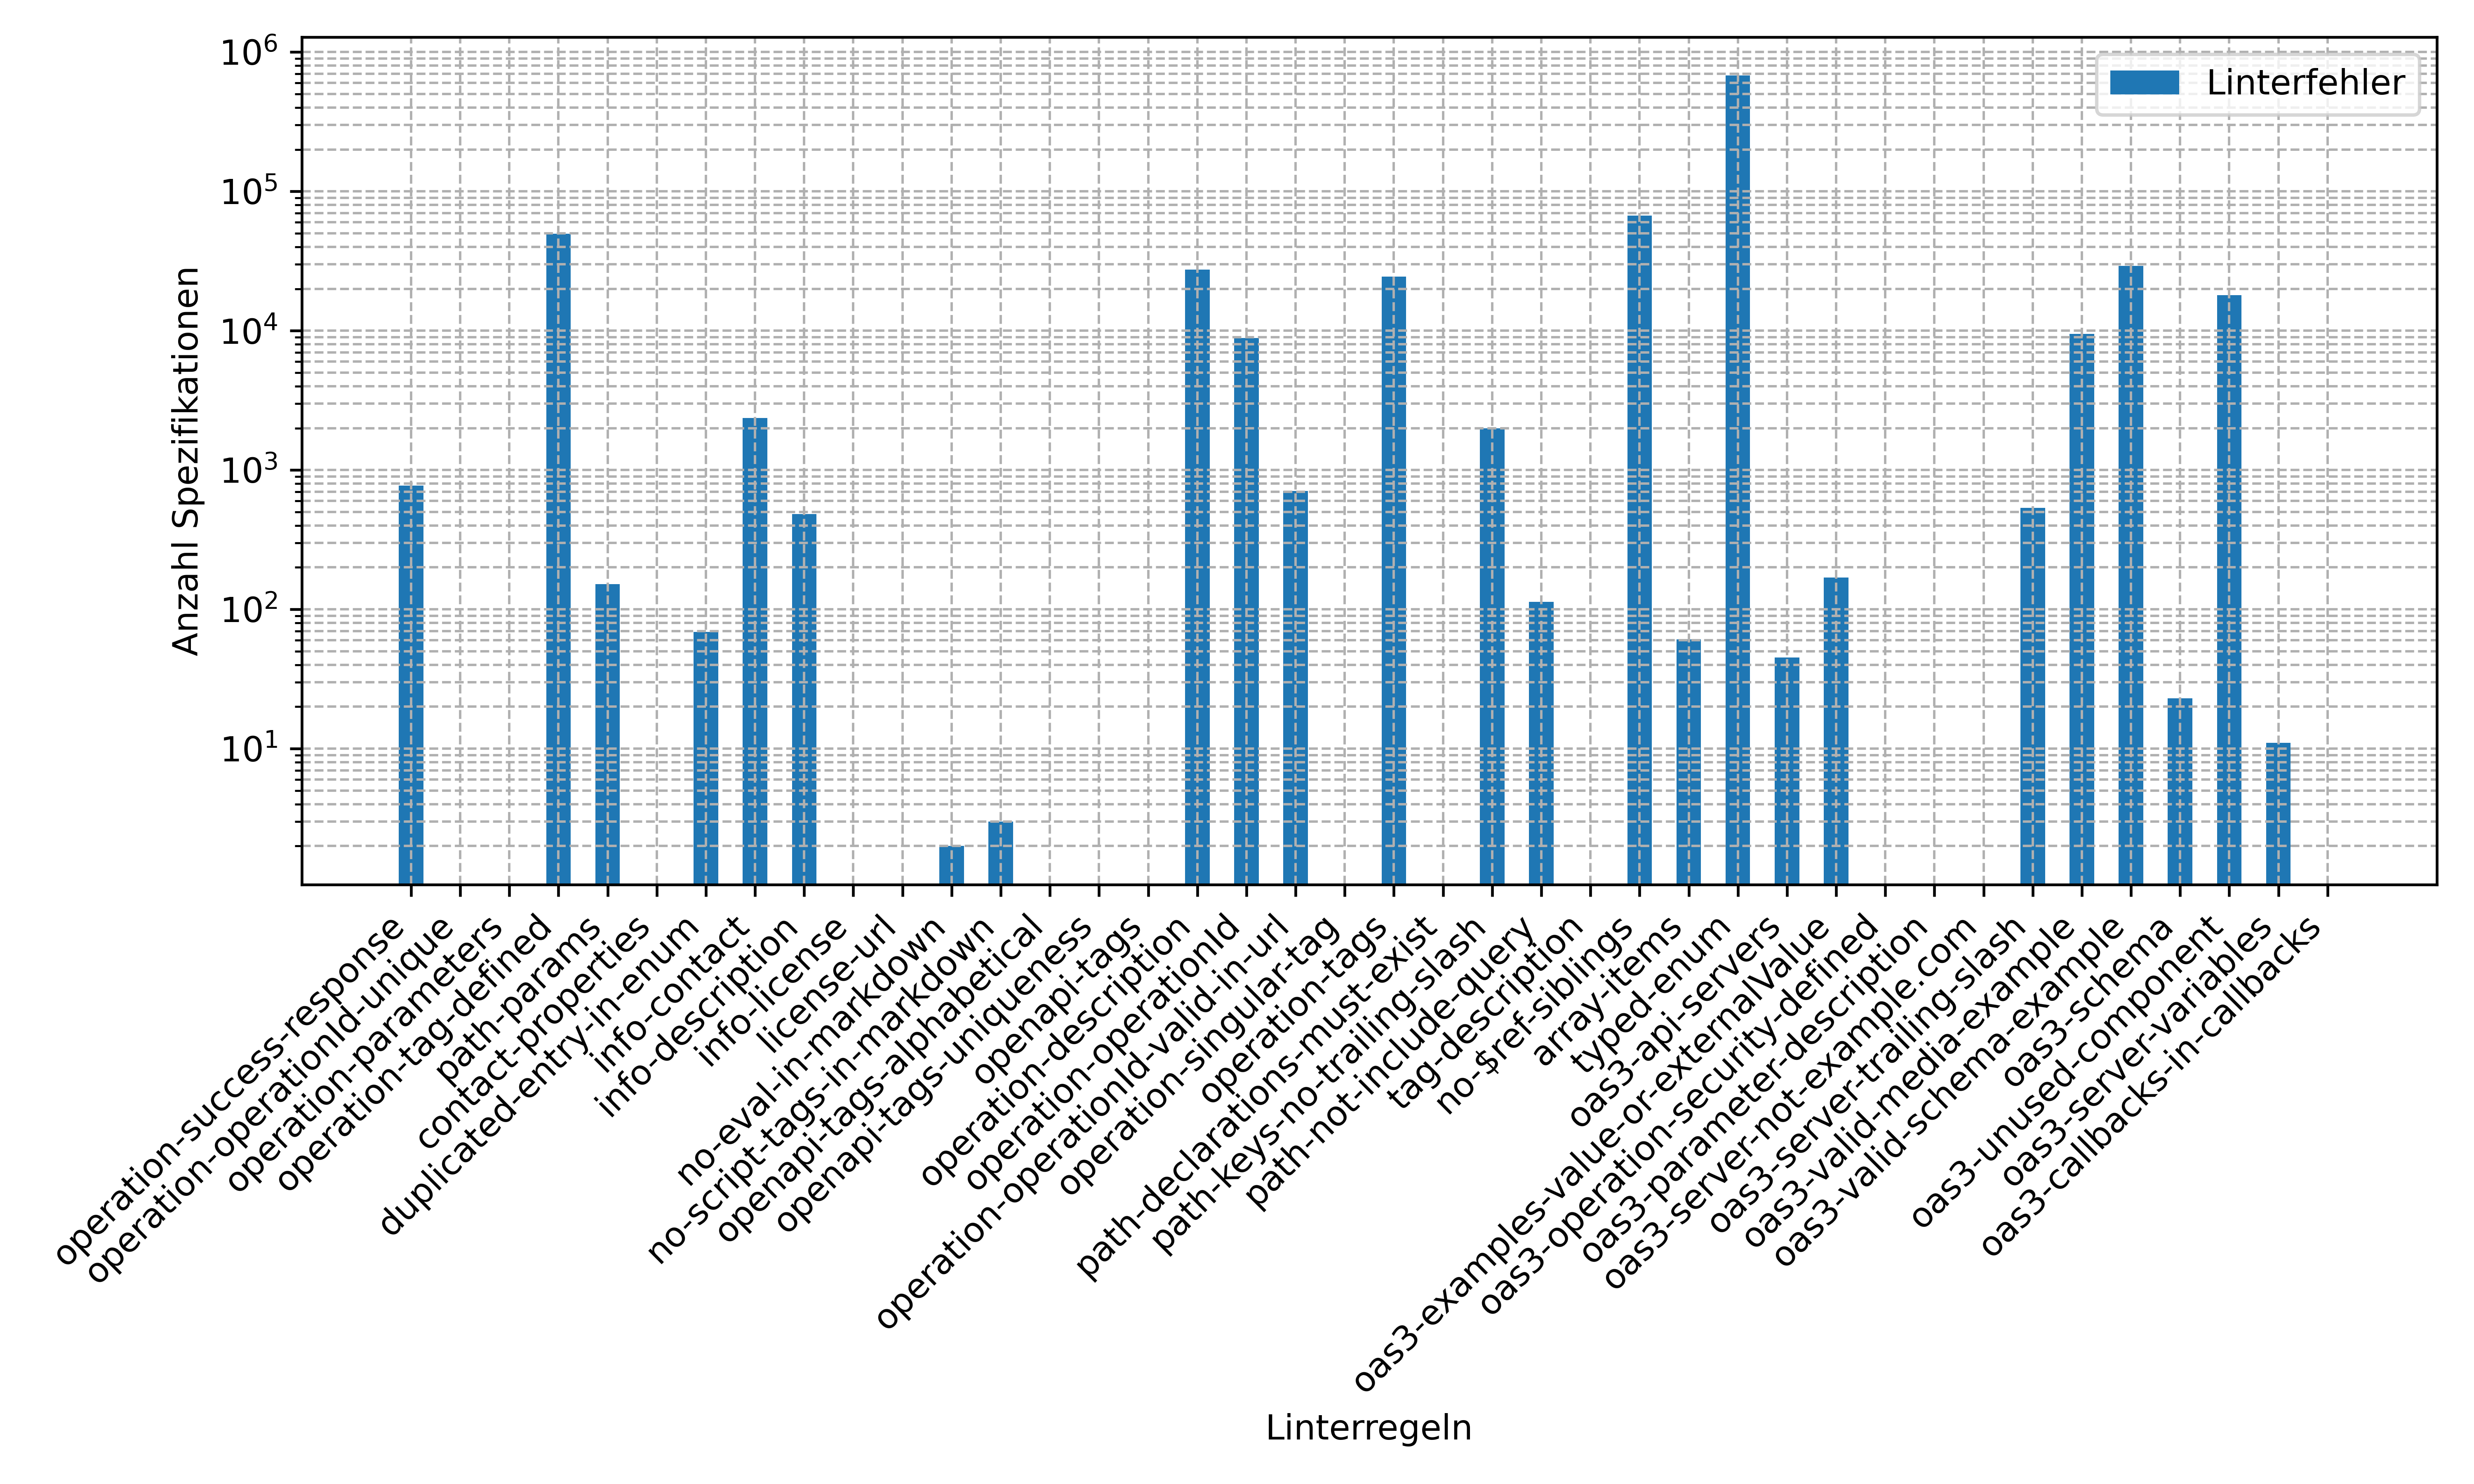
\includegraphics[width=0.85\linewidth]{images/totalspecthrownbarplot.png}
    \caption{Übersicht aller geworfenen Linterfehler}
    \label{fig:totalthrown}
  \end{figure}
\end{frame}

\begin{frame}
  \frametitle{Verzerrung des Datensatzes}
  \begin{itemize}
    \item \textbf{Frage:} Hat die Nutzung des Spectral Linters durch den Anbieter Azure.com einen Einfluss auf die Linterfehler?
    \item \textbf{Methode:} t-Test für unabhängige Stichproben.
    \item \textbf{Ergebnis:} Der durchschnittliche Anteil an Azure.com Linterfehlern ist niedriger, wenn Azure.com die Regel anwendet. 
  \end{itemize}
\end{frame}

\begin{frame}
  \frametitle{Ergebnisse der Invertierung}
  \vspace{-0.4cm}
  \begin{itemize}
    \item Ansatz nur für Single Trigger und Multi Trigger gültig.
    \item Invertierung vielversprechend für genauere Priorisierungen
  \end{itemize}
  \begin{figure}[htbp]
    \centering
    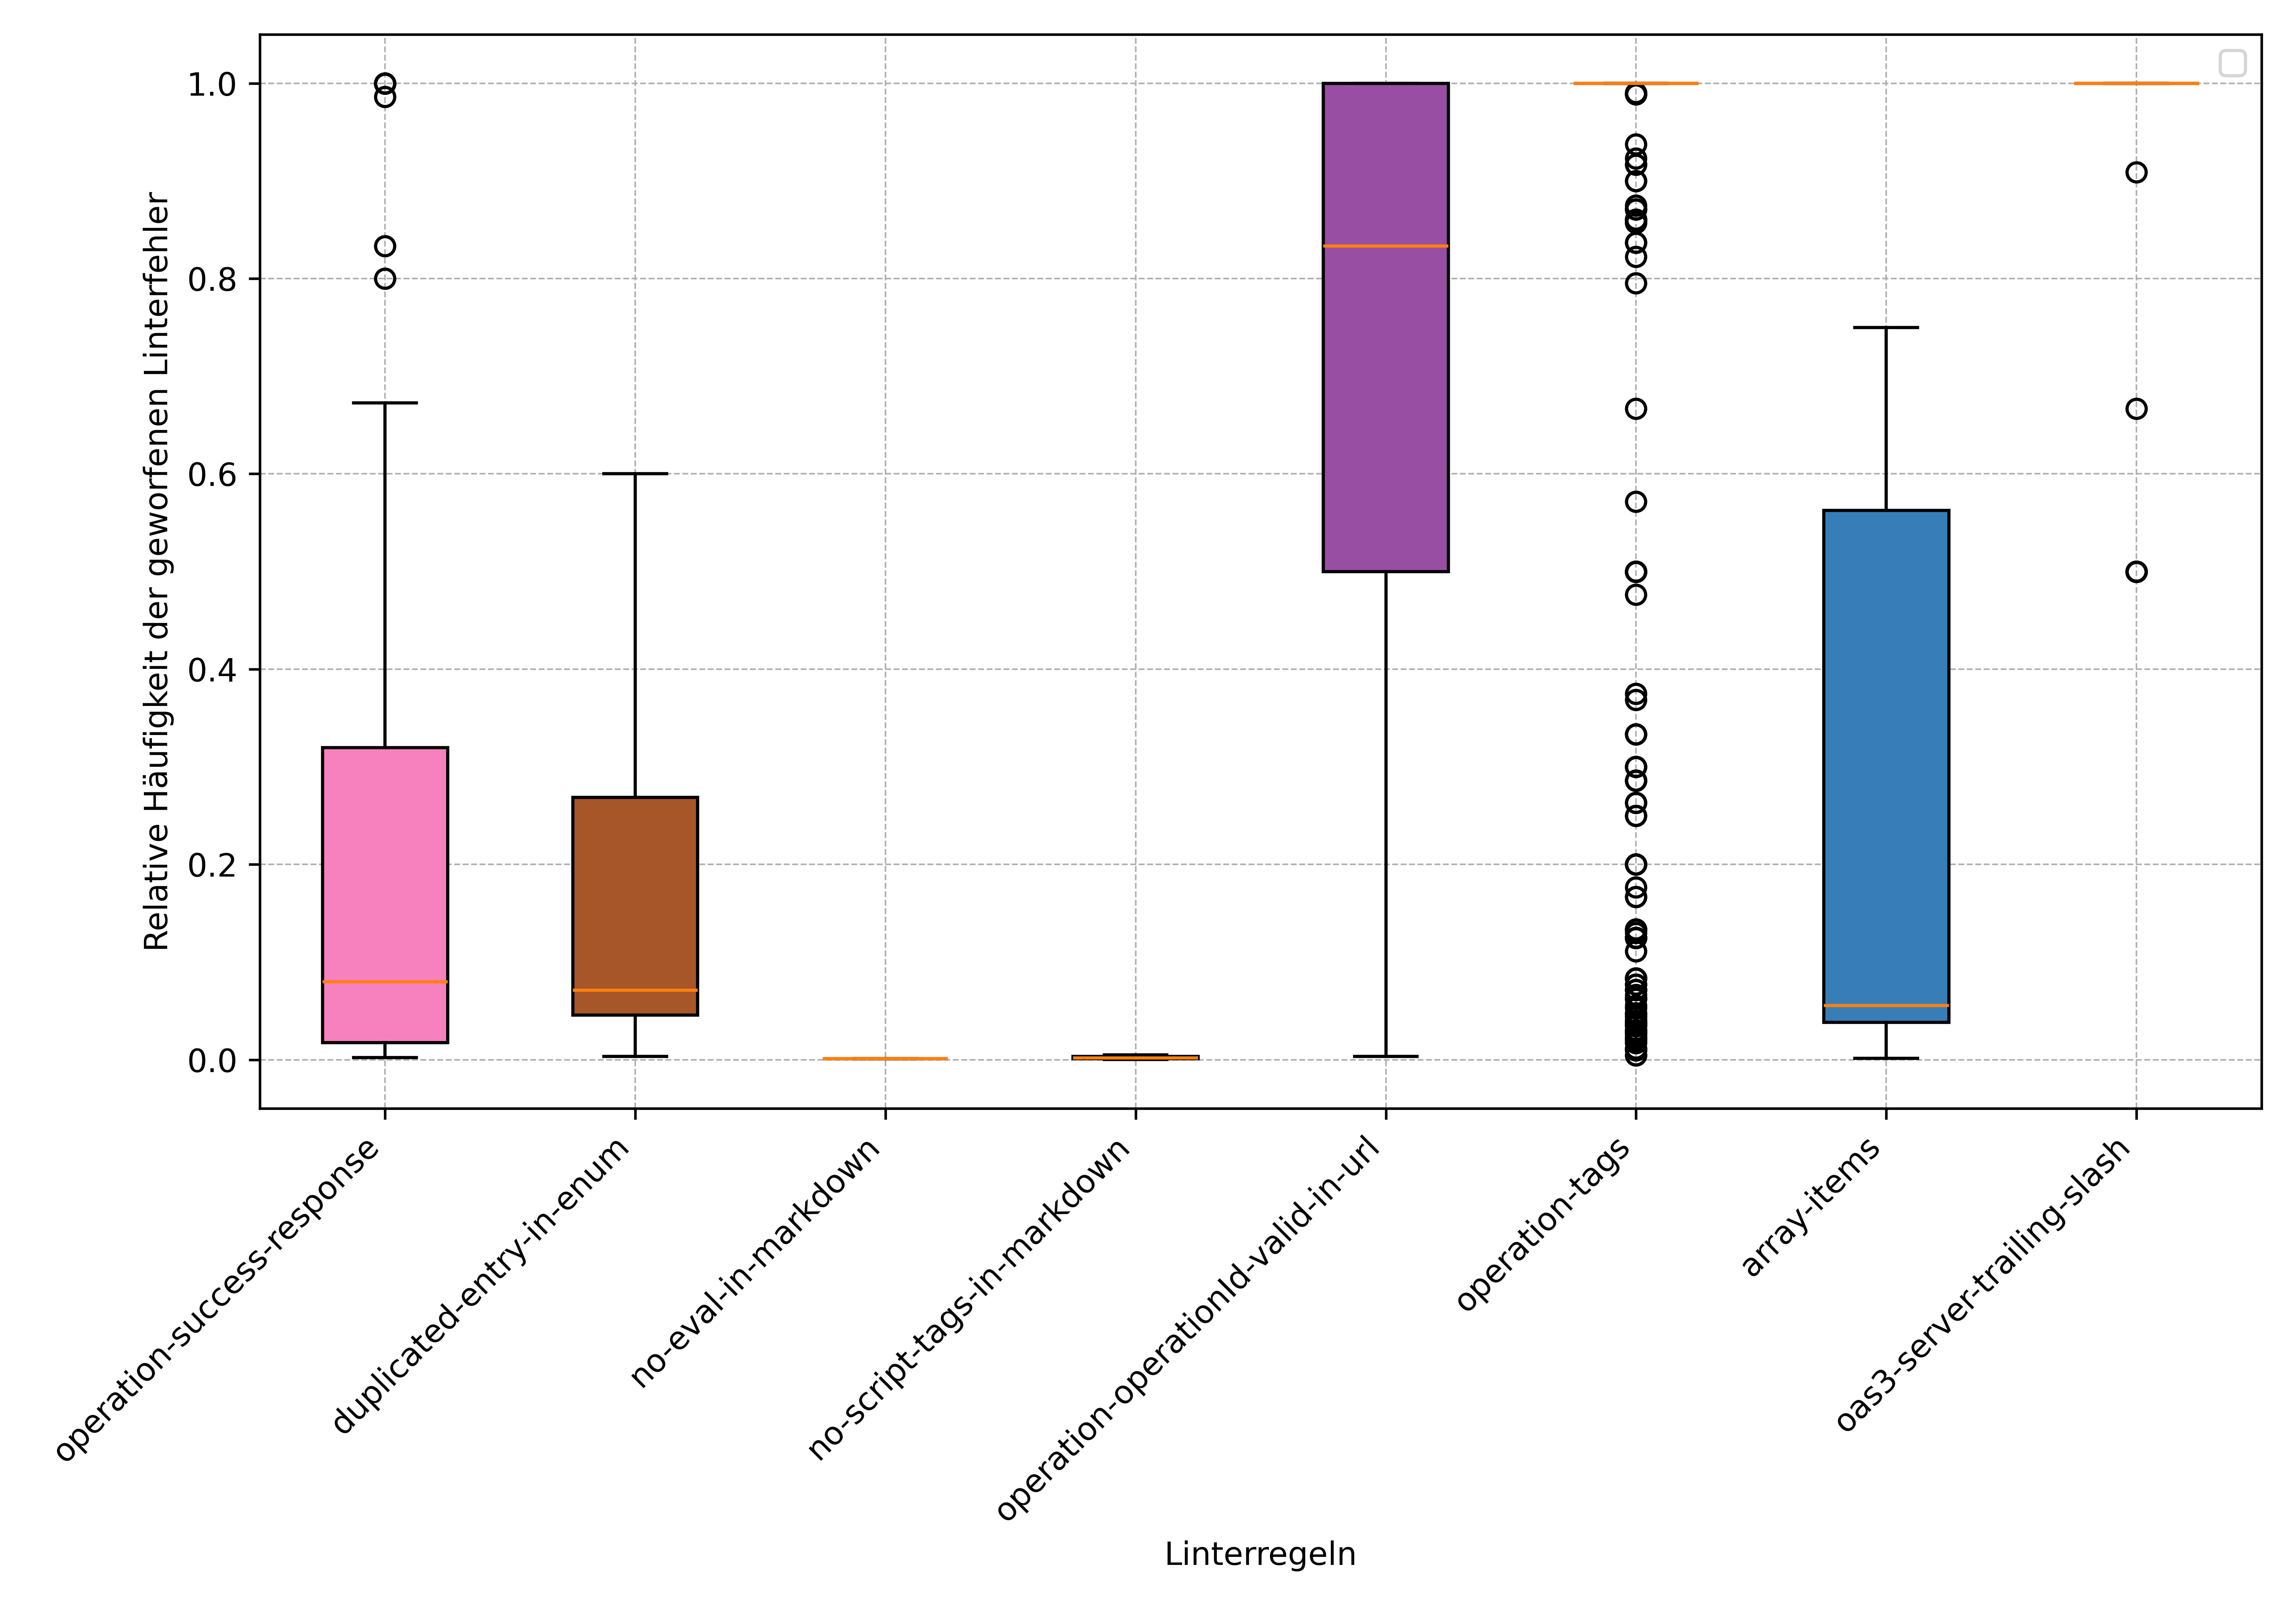
\includegraphics[width=0.75\linewidth]{images/boxplotcleanmultitrigger.png}
    \caption{Multi Trigger Regeln Auslösehäufigkeit}
    \label{fig:boxplot}
  \end{figure}
\end{frame}

\begin{frame}
  \frametitle{Relevanz}
  \vspace{-0.4cm}
  \begin{itemize}
    \item Beide Verfahren teilen Regeln in zwei Gruppen
    \item Regeln, die nie ausgelöst  werden sind am relevantesten
  \end{itemize}
  \begin{figure}[htbp]
    \centering
    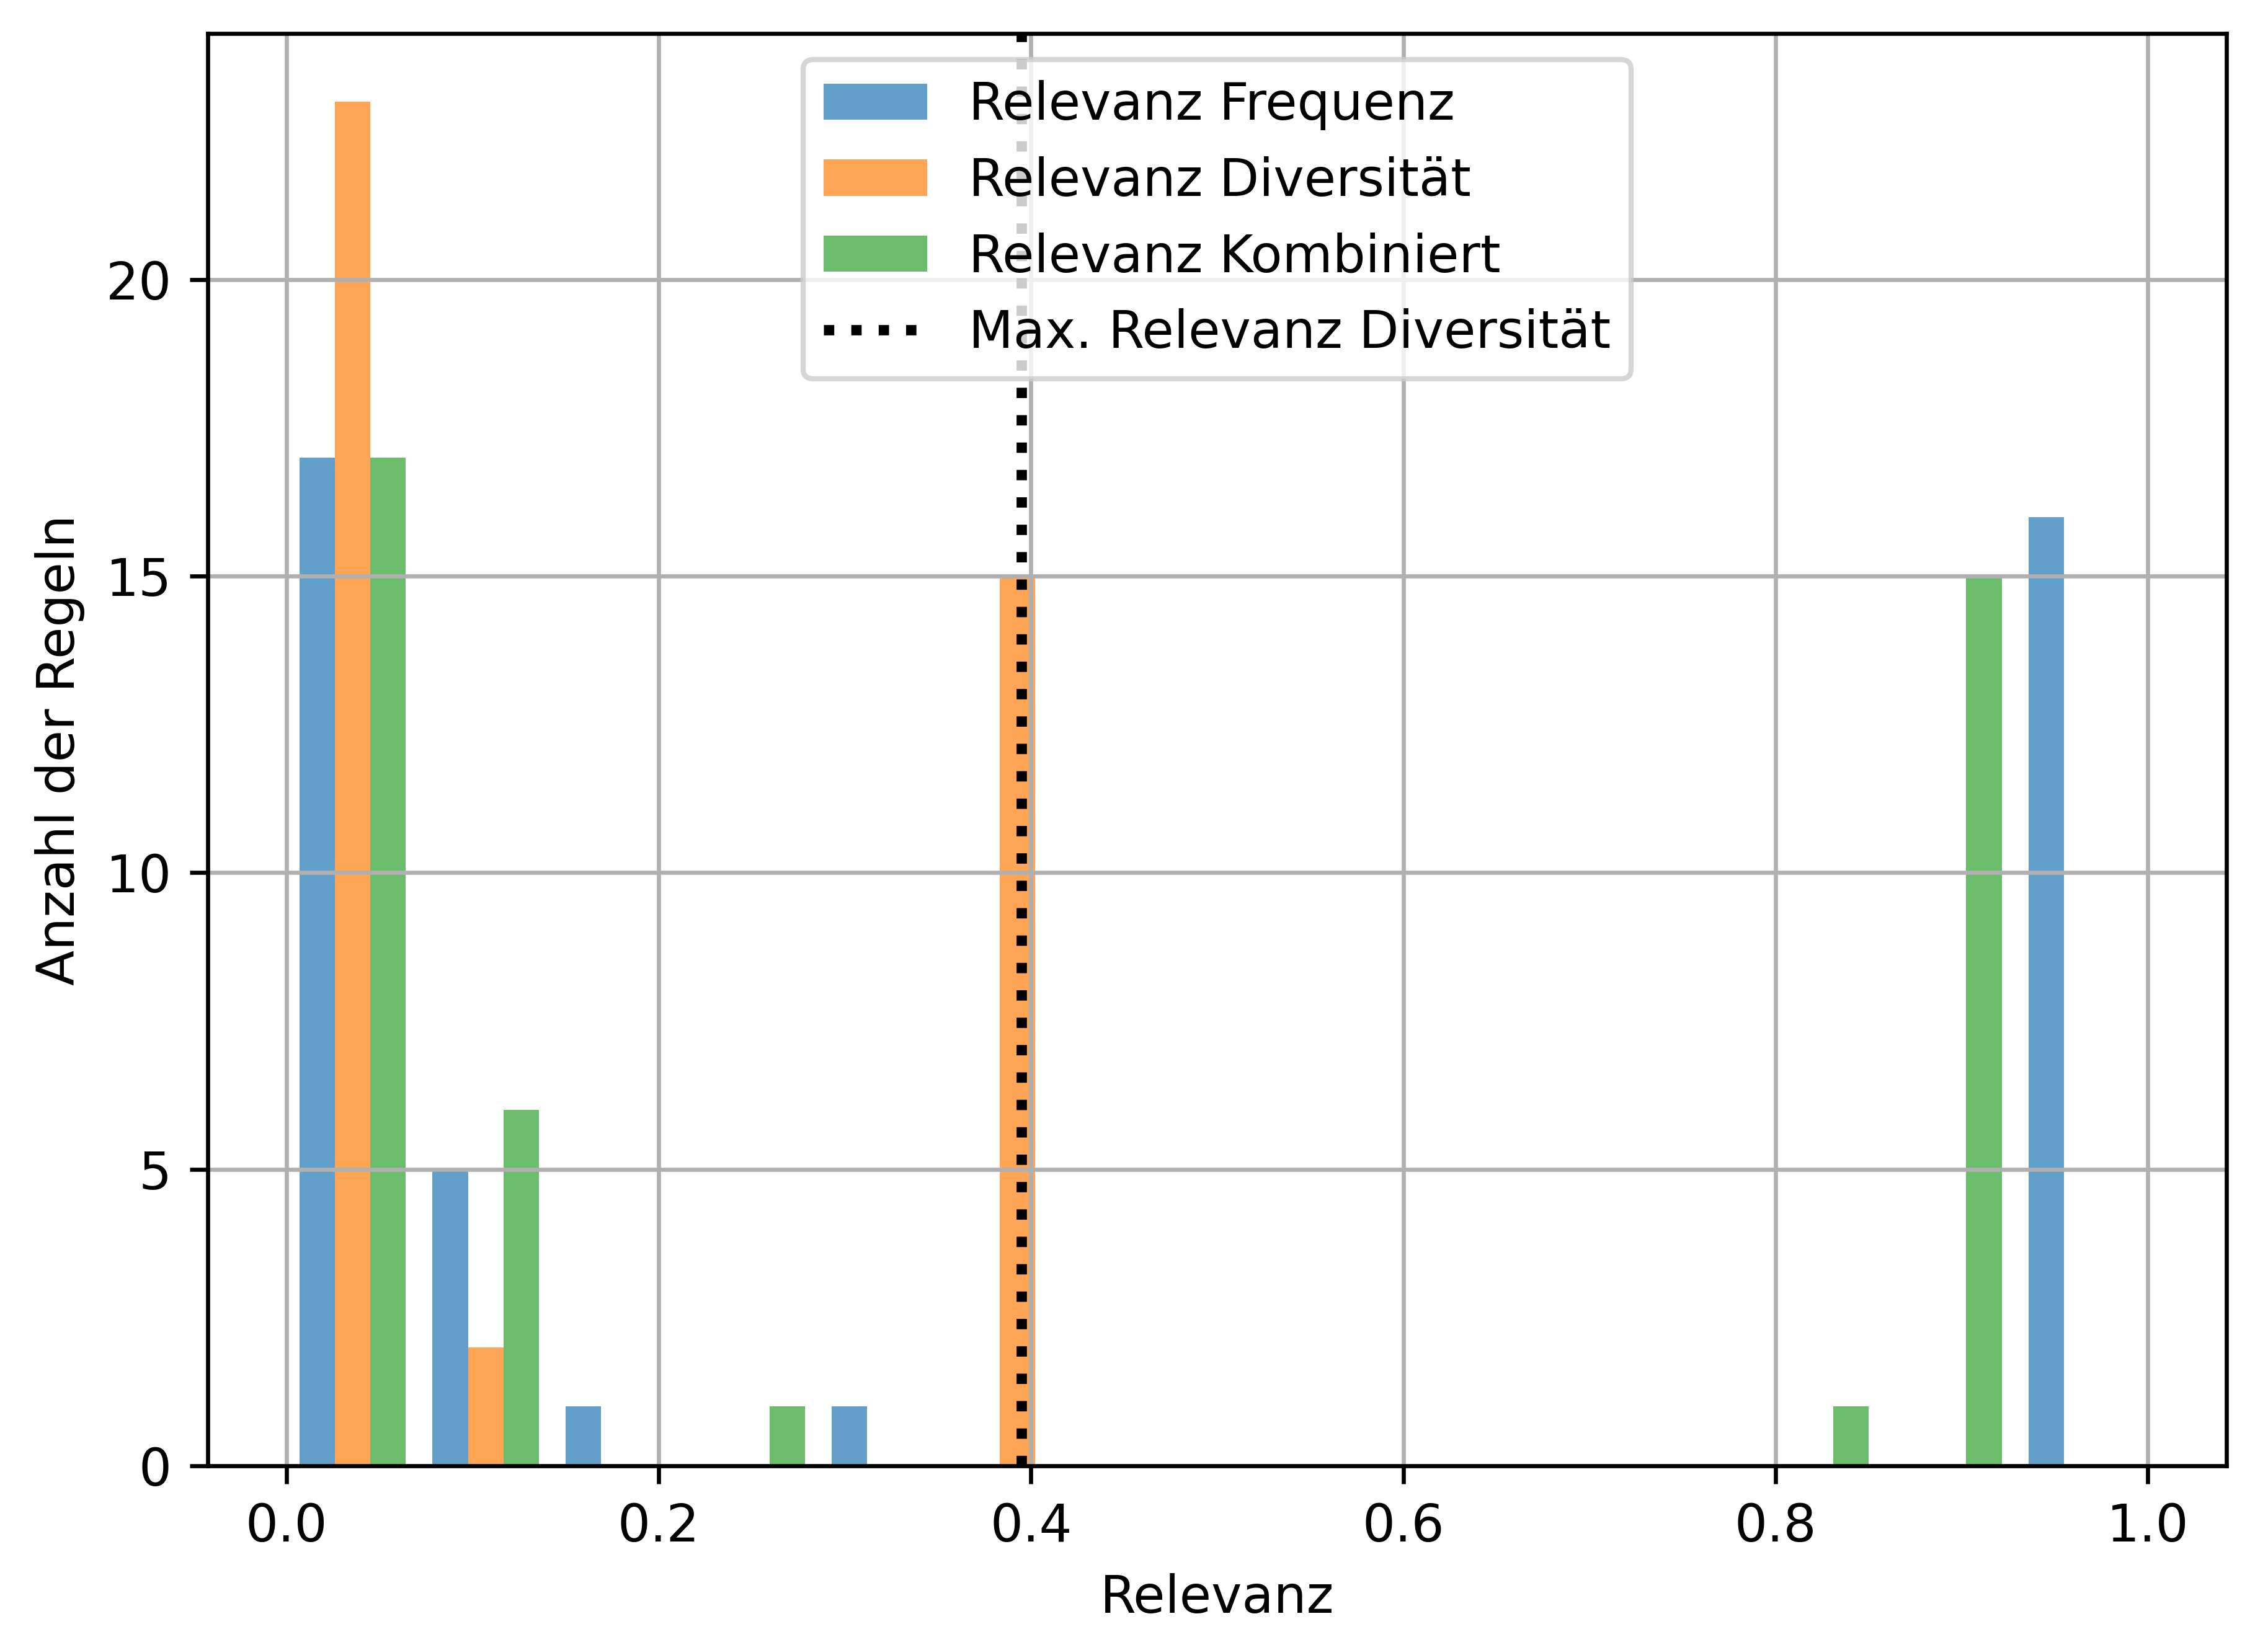
\includegraphics[width=0.78\linewidth]{images/priodistrhist.png}
    \caption{Relevanz der Regeln}
    \label{fig:histogram}
  \end{figure}
\end{frame}

\begin{frame}
  \frametitle{Clustering}
  \vspace{-0.4cm}
  \begin{itemize}
    \item Neuzuordnung der Linterschweregrade mit k-means Clustering
  \end{itemize}
  \begin{figure}[htbp]
    \centering
    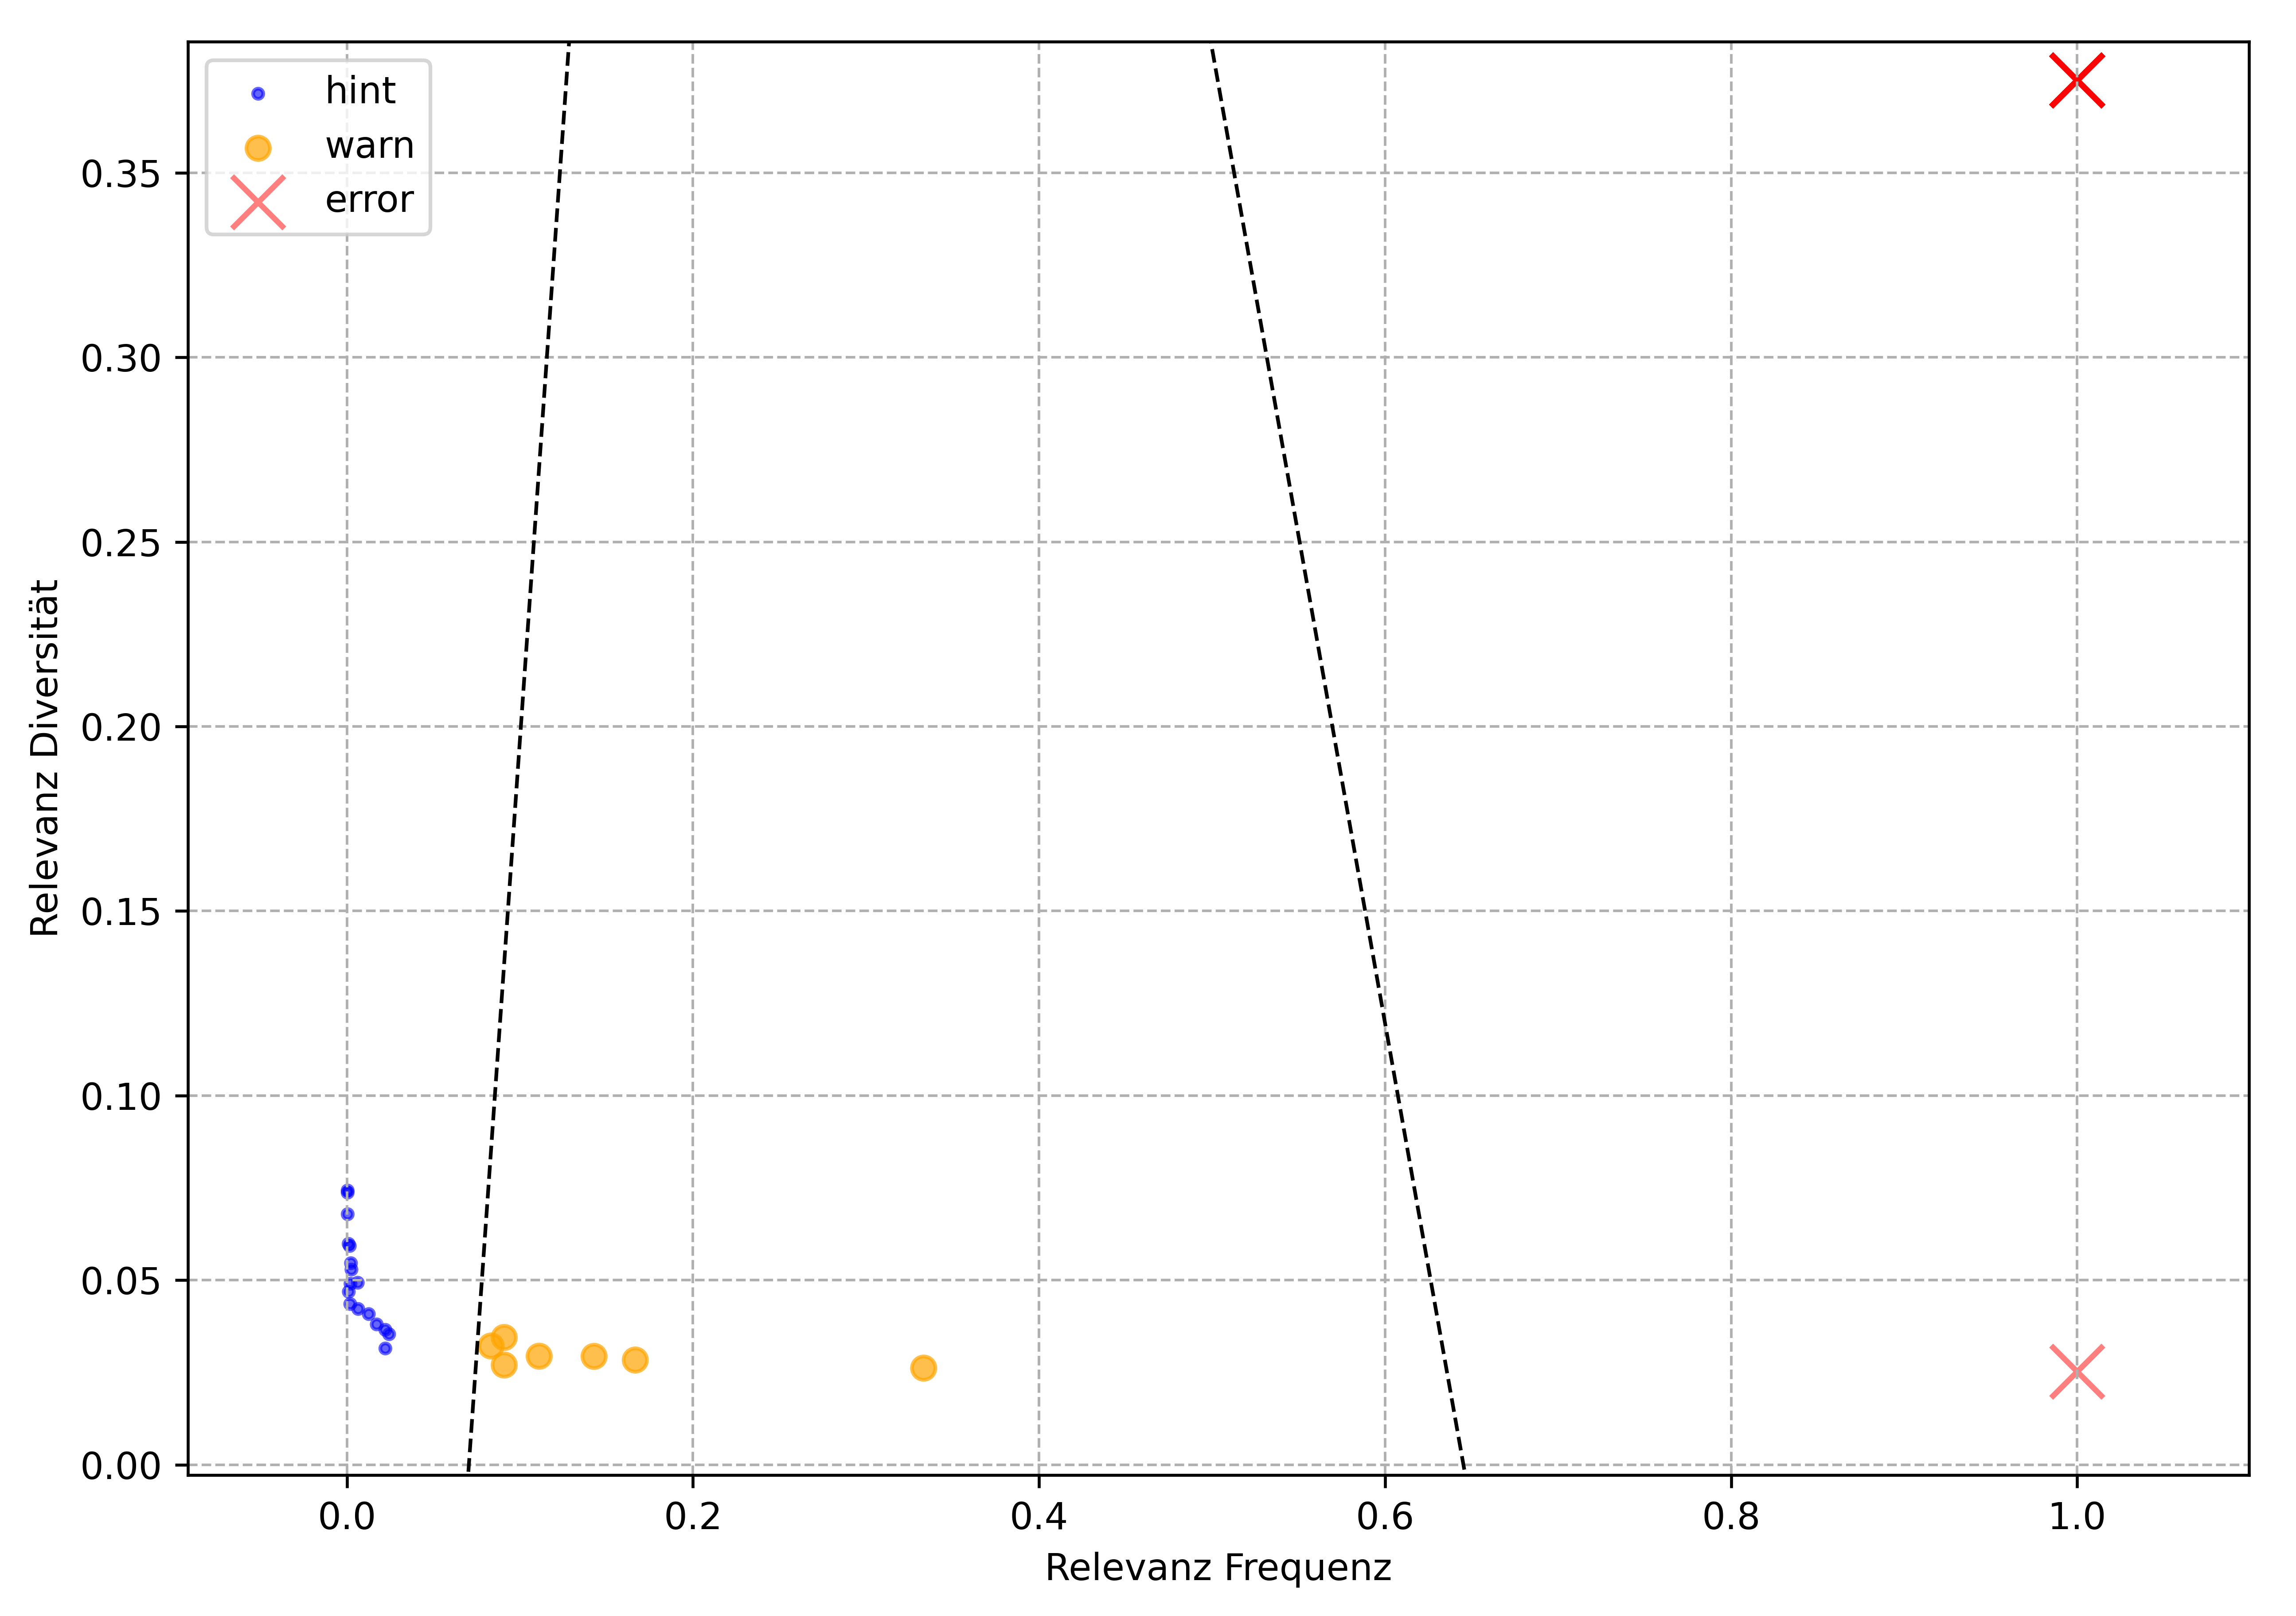
\includegraphics[width=0.8\linewidth]{images/clusterprioscatter.png}
    \caption{Neuzuordnung mit Clustering}
    \label{fig:clustering}
  \end{figure}
\end{frame}

\begin{frame}
  \frametitle{Umverteilung der Schweregrade}
  \begin{longtable}{llr}
    \label{tab:severityreassignments}
    \endfirsthead
    \endhead
    \textbf{Schweregrad OAS} & \textbf{Schweregrad Cluster} & \textbf{Anzahl} \\ \hline
    \texttt{hint} & \texttt{hint} & 4 \\
    \texttt{warn} & \texttt{warn} & 4 \\
    \texttt{error} & \texttt{error} & 1 \\
    \texttt{warn} & \texttt{error} & 13 \\
    \texttt{warn} & \texttt{hint} & 12 \\
    \texttt{hint} & \texttt{warn} & 3 \\
    \texttt{hint} & \texttt{error} & 1 \\
  \caption{Neuverteilungen der Linter Schweregrade}
  \end{longtable}
\end{frame}

\begin{frame}
  \centering{\textbf{Demonstration der Ergebnisse}}
\end{frame}